\documentclass[10pt,a4paper,landscape]{article}

% -- Layout ----
\usepackage[top=0.25cm, bottom=0.25cm, left=0.25cm, right=0.25cm, landscape]{geometry}

% -- Titles ----
\usepackage[
  tiny,                     % text size title
  compact                   % reduce vertical space before/after title
]{titlesec}
% \titlespacing*
\titleformat{\section}{\normalfont\small\bfseries}{\thesection}{0em}{} % Remove space before and after section titles
\titleformat{\subsection}{\normalfont\small\bfseries}{\thesubsection}{0em}{} % Remove space before and after subsection titles
\titlespacing*{\section}{0pt}{0pt}{0pt} % Remove space before/after section titles
\titlespacing*{\subsection}{0pt}{0pt}{0pt} % Remove space before/after subsec titles

% -- Colors ----
\usepackage[dvipsnames]{xcolor}
\definecolor{dmm}{RGB}{192,192,192} % Define a custom dimmed text color

% -- Math ------
\usepackage{mathtools}
\usepackage{amssymb}
\usepackage{turnstile}%better vdash

% -- Lists -----
\usepackage[inline]{enumitem}
\setlist{noitemsep}% Remove vspace between items
% Set vspace before and after  list environments as well as the left margin
\setlist[itemize,1]{leftmargin=*,labelindent=1pt,topsep=1pt,partopsep=1pt}
\setlist[itemize,2]{leftmargin=2pt,labelindent=1pt,topsep=1pt,partopsep=1pt}
\setlist[enumerate,1]{leftmargin=*,labelindent=1pt,topsep=1pt,partopsep=1pt}
\setlist[enumerate,2]{leftmargin=1.2em,labelindent=1pt,topsep=1pt,partopsep=1pt}

% -- Code listing ---
\usepackage{listings}
\lstset{
  aboveskip=3pt,
  belowskip=3pt,
  basicstyle=\small\ttfamily,
  commentstyle=\upshape\ttfamily,
  frame=single,
  language=Haskell,
}

% Parse Trees
\usepackage{tikz}
\usetikzlibrary{ arrows, automata, bbox, calc, positioning }
\tikzset{
% ->, % makes the edges directed
>=stealth', % makes the arrow heads bold
node distance=1cm, % specifies minimum distance between two nodes
% small/.style={},
every state/.style={thick}, % sets the properties for each ’state’ node
every node/.style={inner sep=1pt},
initial text=start, % sets the text that appears on the start arrow
}

% Place a figure env right here via [H] option
\usepackage{float}

% Side by side figure
\usepackage{subcaption}
% \usepackage{caption}
% \captionsetup{belowskip=0pt, aboveskip=0pt}


% -- Multi-Col layout --
\usepackage{multicol}

% -- Global spacing settings ----
% https://lyx-users.lyx.narkive.com/9PDn3r9V/vertical-space-before-and-after-equations
% https://groups.google.com/g/latexusersgroup/c/cXwZxCy29zI?pli=1
% \AtBeginDocument{
% \addtolength{\abovedisplayskip}{-1ex}
% \addtolength{\abovedisplayshortskip}{-1ex}
% \addtolength{\belowdisplayskip}{-1ex}
% \addtolength{\belowdisplayshortskip}{-1ex}
% \addtolength{\textfloatsep}{-2ex}
% \addtolength{\floatsep}{-1ex}
% }
% \setlength{\abovecaptionskip}{-1ex}
% \setlength{\belowcaptionskip}{-1ex}

% No indentation
\setlength\parindent{0pt}

\newcommand{\derive}[2]{\overset{#1}{\underset{#2}{\Rightarrow}}}
\newcommand{\gor}{\;|\;}
\newcommand{\mset}[1]{\(\{q_{#1}\}\)}
\renewcommand{\arraystretch}{1.2}
\newcommand{\xvdash}[1]{%
  \vdash^{\mkern-10mu\footnotesize\rule[-1.2ex]{0pt}{0pt}#1}%
}

\begin{document}
% Suppress page number for all pages
\pagestyle{empty}

\begin{multicols*}{3}

\section*{Grammar, Language, Automata}
{\footnotesize
\begin{tabular}{lp{1cm}p{1.2cm}ll}
  \hline
  G & Langs & Automaton & Productions & Example \\
  \hline
  T-3  & Regular    & DFA/NFA        & \(A \rightarrow \text{a} \& \text{a}B\) & \(L = \{a^{n}\gor n\geq n\}\)\\
  T-2  & CFL   & (N)PDA     & \(A \rightarrow \alpha\) & \(L = \{a^{n}b^{n}\gor n>0\}\)\\
  \textcolor{dmm}{T-1}  & \textcolor{dmm}{Ctx-sst} & \textcolor{dmm}{NDTM} & \textcolor{dmm}{\(\alpha A\beta \rightarrow \alpha\gamma\beta\)} & \textcolor{dmm}{\(L = \{a^{n}b^{n}c^{n}\gor n>0\}\)}\\
  T-0  & RE    & TM        & \(\gamma \rightarrow \alpha\) & \(L = \{w\gor w \text{ desc. } TM\}\)\\
\hline
\end{tabular}
}


\section*{Language of (=accepted by) Automata}
% Language accepted by some Automata
{\footnotesize
\begin{tabular}{l|l}
    $A$utomata & $L$anguage   \\
    \hline
  $\text{DF}A = (Q,\Sigma,\delta,q_{0},F)$
                   & $L(A) = \{w \gor \hat{\delta}(q_{0},w) \in F\}$ \\
  \(\text{NF}A = (Q,\Sigma,\delta,q_{0},F)\)
                   & $L(A) = \{w \gor \hat{\delta}(q_{0},w) \cap F \neq \emptyset\}$\\
  \(\text{PD}A = (Q,\Sigma,\Gamma,\delta,q_{0},F)\)
                   & $L(A) = \{w \gor (q_{0},w,Z_{0}) \underset{P}{\xvdash{*}} (q,\epsilon,\alpha)\}$\\
  \(\text{TM}A = (Q,\Sigma,\Gamma,\delta,q_{0},B,F)\)
                   & $L(A) = \{w \gor (q_{0}w)\xvdash{*} (\alpha p\beta)\}$\\
  \hline
  \multicolumn{2}{l}{$L(A)$ is set of strings $w \in \Sigma^{*}$}\\
  \hline
\end{tabular}
}


\section*{DFA v.s. (\(\epsilon\)-)NFA in 5-tuple form}
{\footnotesize
\begin{tabular}{l|c|c|c}
  \hline
 = & DFA & NFA & \(\epsilon\)-NFA\\
  \hline
 \(Q\) & \multicolumn{3}{c}{finite set of \emph{states}}\\
  \hline
 \(\Sigma\) & \multicolumn{3}{c}{finite set of \emph{input symbols}}\\
  \hline
  \(q_{0}\) & \multicolumn{3}{c}{a \emph{start state} \(\in Q\) } \\
  \hline
  \(\delta\) & \(\delta(q,a) = q \in Q\) & \(\delta(q,a) = \mathsf{S}_{q} \subset Q\) & \(\delta(q,(a\in\Sigma\gor\epsilon)) = \mathsf{S}_{q} \subset Q\)\\
  \hline
 \(F\) & \multicolumn{3}{c}{a set of \emph{final} or \emph{accepting} states \(\subset Q\)}\\
\hline
\end{tabular}
}


\section*{DFA: tuple, transition diagram, transition table}
{\footnotesize\(L\) accepted by following DFA: \(x01y\)\hfill ({\(x,y\) are any strings of 0's/1's})
\vspace{-0.5em}
  \[
A_{\text{DFA}} = (\{q_{0},q_{1},q_{2}\},\{0,1\},\delta,q_{0},\{q_{1}\})
  \]
\begin{minipage}[b]{0.45\linewidth}
  \centering
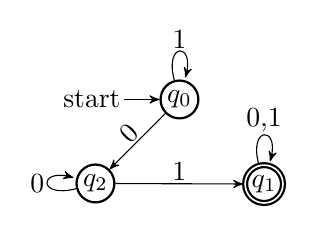
\begin{tikzpicture}[bezier bounding box]%reduce vertical space around graph
  \node[state, initial, minimum size=1em] (q0) {$q_0$};
  \node[state, minimum size=1em, below left=of q0] (q2) {$q_2$};
  \node[state, accepting, minimum size=1em, below right=of q0] (q1) {$q_{1}$};

  \path[->]
  (q0) edge[loop above] node{1}(q0)
       edge node[above,sloped]{0} (q2)

  (q2) edge[loop left] node{0}(q2)
       edge node[above]{1}(q1)

  (q1) edge[loop above] node{0,1}(q1);
\end{tikzpicture}\\
DFA transition diagram
\end{minipage}
\begin{minipage}[b]{0.45\linewidth}
\centering
\begin{tabular}{r||c|c}
   & 0 & 1 \\
  \hline
  \(\rightarrow q_{0}\) & \(q_{2}\) & \(q_{0}\)\\
  \(*q_{1}\) & \(q_{1}\) & \(q_{1}\)\\
  \(q_{2}\) & \(q_{2}\) & \(q_{1}\)\\
  \hline
\end{tabular}\\
\vskip 1em
DFA transition table
\end{minipage}
}


\section*{NFA: tuple, transition diagram, transition table}
{\footnotesize\(L\) accepted by following NFA: \(x01\)\hfill (any strings ending in 01)
\vspace{-0.5em}
  \[
A_{\text{NFA}} = (\{q_{0},q_{1},q_{2}\},\{0,1\},\delta,q_{0},\{q_{2}\})
  \]
  \begin{minipage}[b]{0.45\linewidth}
    \centering
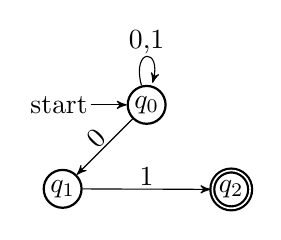
\begin{tikzpicture}[bezier bounding box]%reduce vertical space around graph
  \node[state, initial, minimum size=1em] (q0) {$q_{0}$};
  \node[state, minimum size=1em, below left=of q0] (q1) {$q_{1}$};
  \node[state, accepting, minimum size=1em, below right=of q0] (q2) {$q_{2}$};

  \path[->]
  (q0) edge[loop above] node{0,1}(q0)
       edge node[above,sloped]{0} (q1)
  (q1) edge node[above]{1}(q2)
  (q2);
\end{tikzpicture}\\
NFA transition diagram
\end{minipage}
\begin{minipage}[b]{0.45\linewidth}
\centering
\begin{tabular}{r||c|c}
   & 0 & 1 \\
  \hline
  \(\rightarrow q_{0}\) & \(\{q_{0},q_{1}\}\) & \(\{q_{0}\}\)\\
  \(q_{1}\) & \(\emptyset\) & \(\{q_{2}\}\)\\
  \(*q_{2}\) & \(\emptyset\) & \(\emptyset\)\\
  \hline
\end{tabular}\\
\vskip 1em
NFA transition table
\end{minipage}
}


\section*{NFA to DFA (subset construction)}
At worst, NFA$_{n\text{-states}}$ converts to DFA$_{2^{n}\text{-states}}$\\
\vspace{-0.5em}
{\footnotesize
\[
  N_{\text{NFA}} = (Q_{N},\Sigma,\delta_{N},\mathbf{q_{0}},F_{N}) \Rightarrow (Q_{D},\Sigma,\delta_{D},{\mathbf{\{q_{0}\}}},F_{D}) = D_{\text{DFA}}
\]
}
% subset construction steps
{\footnotesize
\begin{minipage}{0.5\linewidth}
Extend NFA transition table (ref)
  \begin{enumerate}[align=left]
    \item\label{nfa:sub} Find \textbf{sets of states} that NFA's \(\{q_{0}\}\),\(\{q_{1}\}\)\ldots\(\{q_{n }\}\) can reach
    \item If any \textbf{new state set} in step \ref{nfa:sub}, see what \textbf{state set} it can reach
    \item Unreachable/dead states marked by \(\emptyset\)  (``thrown away'')
    \item If any state set found above has any \(q_{i} \in F_{N}\), mark the set with *
    \item (optional) mark state sets as \(S_{0\ldots i}\) and draw NFA transition diagram
  \end{enumerate}
\end{minipage}%
\begin{minipage}{0.45\linewidth}
  \centering
\begin{tabular}{r||c|c}
   & 0 & 1 \\
  \hline
  \(\emptyset\) & \(\emptyset\) & \(\emptyset\)\\
  \(\rightarrow \{q_{0}\}\) & \(\{q_{0},q_{1}\}\) & \(\{q_{0}\}\)\\
  \(\{q_{1}\}\) & \(\emptyset\) & \(\{q_{2}\}\)\\
  \(*\{q_{2}\}\) & \(\emptyset\) & \(\emptyset\)\\
  \(\{q_{0},q_{1}\}\) & \(\{q_{0},q_{1}\}\) & \(\{q_{0},q_{2}\}\)\\
  \(*\{q_{0},q_{2}\}\) & \(\{q_{0},q_{1}\}\) & \(\{q_{0}\}\)\\
  \(*\{q_{1},q_{2}\}\) & \(\emptyset\) & \(\{q_{0}\}\)\\
  \(*\{q_{0},q_{1},q_{2}\}\) & \(\{q_{0},q_{1}\}\) & \(\{q_{0},q_{2}\}\)\\
  \hline
\end{tabular}
\end{minipage}
}


\section*{\(\epsilon\)-closures of state(s)}
{\footnotesize
% enumerate env better to use default c
% tikz env better to use t or b
\begin{minipage}{0.4\linewidth}
  \begin{enumerate}
    \item state \(q\) itself is in \textsc{eclose}(\(q\))
    \item\label{nfa:epi1} following all \(epsilon\) transitions out of \(q\)
    \item\label{nfa:epi2} each of \(q\)'s \(epsilon\) reachable state \(p_{q\text{-}\epsilon}\) is in \textsc{eclose}(\(q\))
    \item each of \(p_{q\text{-}\epsilon}\)'s  \(epsilon\) reachable state \(r_{p\text{-}\epsilon}\) is in \textsc{eclose}(\(q\))
    \item for state set \(S\), do above steps 1-4 for each in \(S\) and take the union
  \end{enumerate}
\end{minipage}%
\begin{minipage}{0.55\linewidth}
  \centering
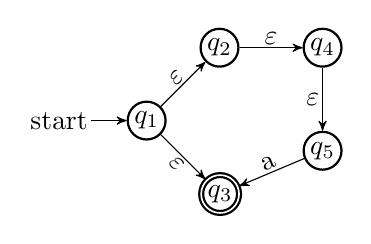
\begin{tikzpicture}[bezier bounding box,node distance=0.8cm]%reduce vertical space around graph
  \node[state, initial, minimum size=0.8em] (q1) {$q_{1}$};
  \node[state, minimum size=0.8em, above right=of q1] (q2) {$q_{2}$};
  \node[state, minimum size=0.8em, right=of q2] (q4) {$q_{4}$};
  \node[state, minimum size=0.8em, below=of q4] (q5) {$q_{5}$};
  \node[state, accepting, minimum size=0.5em, below right=of q1] (q3) {$q_{3}$};

  \path[->]
  (q1) edge node[above,sloped]{\(\varepsilon\)}(q2)
  (q1) edge node[below,sloped]{\(\varepsilon\)}(q3)
  (q2) edge node[above]{\(\varepsilon\)}(q4)
  (q4) edge node[left]{\(\varepsilon\)}(q5)
  (q5) edge node[above,sloped]{a}(q3);
\end{tikzpicture}\\
\textsc{eclose}(\(q_{1}\))=\(\{q_{1},q_{2},q_{3},q_{4},q_{5}\}\)
\end{minipage}
}


\section*{Remove \(\epsilon\)-Transitions (\(epsilon\)-NFA to DFA)}
{\footnotesize
% better to make left enumerate higher than right graph
\begin{minipage}{0.45\linewidth}
  \begin{enumerate}[align=left]
    \item \(\epsilon\)-close each states in \(Q_{E}\)
    \item For any \(q_{i} \in Q_{E}\), if \textsc{eclose}(\(q\)) contains any \(q_{i} \in F_{E}\), then \(q\) be a \emph{final/accepting} state in result DFA
    \item\label{nfa:erem} Check if any \(q_{i}\) in \textsc{eclose}(\(q\)) meet: \(\delta(q_{i},a) = s \rightarrow \delta(q,a) = s\) where \(s \in Q\)
    \item (optional) \textbf{copy} orig \(\epsilon\)-NFA diagram, \textbf{erase} all \(\epsilon\)-transitions and show connections found in step \ref{nfa:erem} in result DFA
    \item (optional) ignore all dead states \(\emptyset\) and transitions to them (avoid clutter)
  \end{enumerate}
\end{minipage}%
\begin{minipage}{0.5\linewidth}
\centering
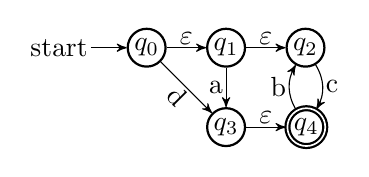
\begin{tikzpicture}[bezier bounding box,node distance=0.5cm]%reduce vertical space around graph
  \node[state, initial, minimum size=0.5em] (q0) {$q_{0}$};
  \node[state, minimum size=0.5em, right=of q0] (q1) {$q_{1}$};
  \node[state, minimum size=0.5em, right=of q1] (q2) {$q_{2}$};
  \node[state, minimum size=0.5em, below=of q1] (q3) {$q_{3}$};
  \node[state, accepting, minimum size=0.5em, right=of q3] (q4) {$q_{4}$};

  \path[->]
  (q0) edge node[above]{\(\varepsilon\)}(q1)
  (q0) edge node[below,sloped]{d}(q3)
  (q1) edge node[above]{\(\varepsilon\)}(q2)
  (q1) edge node[left]{a}(q3)
  (q2) edge[bend left] node[right]{c}(q4)
  (q3) edge node[above]{\(\varepsilon\)}(q4)
  (q4) edge[bend left] node[left]{b}(q2);
\end{tikzpicture}
\vspace{1em}\\
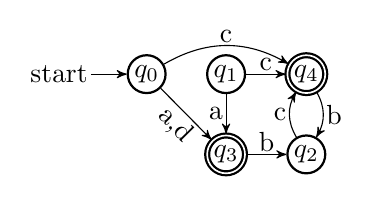
\begin{tikzpicture}[bezier bounding box,node distance=0.5cm]%reduce vertical space around graph
  \node[state, initial, minimum size=0.8em] (q0) {$q_{0}$};
  \node[state, minimum size=0.8em, right=of q0] (q1) {$q_{1}$};
  \node[state, accepting, minimum size=0.8em, below=of q1] (q3) {$q_{3}$};
  \node[state, minimum size=0.8em, right=of q3] (q2) {$q_{2}$};
  \node[state, accepting, minimum size=0.5em, right=of q1] (q4) {$q_{4}$};

  \path[->]
  (q0) edge node[below,sloped]{a,d}(q3)
  (q0) edge[bend left] node[above]{c}(q4)
  (q1) edge node[above]{c}(q4)
  (q1) edge node[left]{a}(q3)
  (q2) edge[bend left] node[left]{c}(q4)
  (q3) edge node[above]{b}(q2)
  (q4) edge[bend left] node[right]{b}(q2);
\end{tikzpicture}
\end{minipage}
}


\section*{Regular Expressions to $\epsilon$-NFA}
\begin{enumerate}
\item $LM$ or $L.M$ = $\{wx\}$ for any $w \in L \wedge x \in M$ (concat)
\item $a^{*}$ 0 or more of a (Kleene star)
\item $a^{+}$ 1 or more of a
\item $a\gor b$ either a or b ($0+1$, union)
\item $(01)1$ (first 0 and 1 are grouped)
\item $\epsilon$ empty string
\end{enumerate}
\vspace{-1em}
{\footnotesize
% R1R2
\begin{minipage}{0.4\linewidth}
\centering
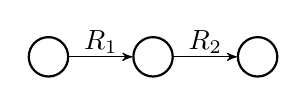
\begin{tikzpicture}[bezier bounding box,node distance=0.8cm]%reduce vertical space around graph
  \node[state, minimum size=0.5cm] (s0) {};
  \node[state, minimum size=0.5cm, right=of s0] (s1) {};
  \node[state, minimum size=0.5cm, right=of s1] (s2) {};

  \path[->]
  (s0) edge node[above]{$R_{1}$}(s1)
  (s1) edge node[above]{$R_{2}$}(s2);
\end{tikzpicture}\\
Regex of $R_{1}R_{2}$
\end{minipage}
% R*
\begin{minipage}{0.55\linewidth}
\centering
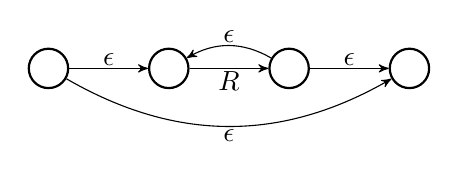
\begin{tikzpicture}[bezier bounding box,node distance=1cm]%reduce vertical space around graph
  \node[state, minimum size=0.5cm] (s0) {};
  \node[state, minimum size=0.5cm, right=of s0] (s1) {};
  \node[state, minimum size=0.5cm, right=of s1] (s2) {};
  \node[state, minimum size=0.5cm, right=of s2] (s3) {};

  \path[->]
  (s0) edge node[above]{$\epsilon$}(s1)
  (s0) edge[bend right] node[below]{$\epsilon$}(s3)
  (s1) edge node[below]{$R$}(s2)
  (s2) edge node[above]{$\epsilon$}(s3)
  (s2) edge[bend right] node[above]{$\epsilon$}(s1);
\end{tikzpicture}\\
Regex of $R^{*}$
\end{minipage}
\begin{minipage}{0.4\linewidth}
\centering
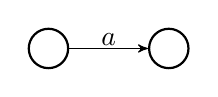
\begin{tikzpicture}[bezier bounding box]%reduce vertical space around graph
  \node[state, minimum size=0.5cm] (s0) {};
  \node[state, minimum size=0.5cm, right=1cm of s0] (s1) {};

  \path[->] (s0) edge node[above]{$a$}(s1);
\end{tikzpicture}\\
Regex a, language \{a\}

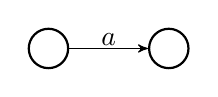
\begin{tikzpicture}[bezier bounding box]%reduce vertical space around graph
  \node[state, minimum size=0.5cm] (s0) {};
  \node[state, minimum size=0.5cm, right=1cm of s0] (s1) {};

  \path[->]
  (s0) edge node[above]{$a$}(s1);
\end{tikzpicture}\\
Regex $\epsilon$, language $\{\epsilon\}$

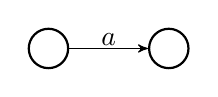
\begin{tikzpicture}[bezier bounding box]%reduce vertical space around graph
  \node[state, minimum size=0.5cm] (s0) {};
  \node[state, minimum size=0.5cm, right=1cm of s0] (s1) {};

  \path[->] (s0) edge node[above]{$a$}(s1);
\end{tikzpicture}\\
Regex $\emptyset$, language $\emptyset$
\end{minipage}
% R1|R2
\begin{minipage}{0.5\linewidth}
\centering
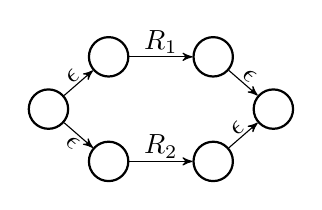
\begin{tikzpicture}[bezier bounding box,node distance=0.8cm]%reduce vertical space around graph
  \node[state, minimum size=0.5cm] (s1) {};
  \node[state, minimum size=0.5cm, right=of s1] (s2) {};
  \node[state, minimum size=0.5cm, below=of s1] (s3) {};
  \node[state, minimum size=0.5cm, right=of s3] (s4) {};

  % Calculate the midpoint between S1 and S3
  \coordinate (mid13) at ($(s1)!0.5!(s3)$);
  \node[state, minimum size=0.5cm, left=0.5cm of mid13] (s0) {};

  % Calculate the midpoint between S2 and S4
  \coordinate (mid24) at ($(s2)!0.5!(s4)$);
  \node[state, minimum size=0.5cm, right=0.5cm of mid24] (s5) {};

  \path[->]
  (s0) edge node[above,sloped]{$\epsilon$}(s1)
  (s0) edge node[below,sloped]{$\epsilon$}(s3)
  (s1) edge node[above]{$R_{1}$}(s2)
  (s2) edge node[above,sloped]{$\epsilon$}(s5)
  (s3) edge node[above]{$R_{2}$}(s4)
  (s4) edge node[above,sloped]{$\epsilon$}(s5);
\end{tikzpicture}\\
Regex of $R_{1}|R_{2}$
\end{minipage}
}
\begin{minipage}{\linewidth}
  \centering
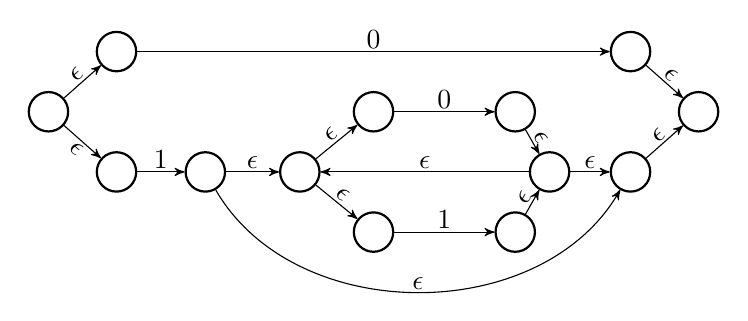
\begin{tikzpicture}[bezier bounding box]%reduce vertical space around graph
  % Outer circle 0|1 ---------------------------------
  \node[state, minimum size=0.5cm] (s2) {};
  \node[state, minimum size=0.5cm, right=6cm of s2] (s3) {};
  \node[state, minimum size=0.5cm, below=of s2] (s5) {};
  \node[state, minimum size=0.5cm, right=6cm of s5] (s6) {};

  % Calculate the midpoint between S2 and S5
  \coordinate (mid25) at ($(s2)!0.5!(s5)$);
  \node[state, minimum size=0.5cm, left=0.6cm of mid25] (s1) {};

  % Calculate the midpoint between S3 and S6
  \coordinate (mid36) at ($(s3)!0.5!(s6)$);
  \node[state, minimum size=0.5cm, right=0.6cm of mid36] (s4) {};

  % Inner circle (0|1)* ------------------------------
  \node[state, minimum size=0.5cm, right=3cm of mid25] (s8) {};
  \node[state, minimum size=0.5cm, left=1.2cm of mid36] (s9) {};
  \node[state, minimum size=0.5cm, below=of s9] (s11) {};
  \node[state, minimum size=0.5cm, below=of s8] (s12) {};

  % 7/10 special
  \node[state, minimum size=0.5cm, right=1.8cm of s5] (s7) {};
  \node[state, minimum size=0.5cm, left=0.5cm of s6]  (s10) {};

  % 13 special
  \node[state, minimum size=0.5cm, right=0.6cm of s5] (s13) {};

  % Calculate the midpoint between S8 and S12
  % \coordinate (mid812) at ($(s8)!0.5!(s12)$);
  % \node[state, minimum size=0.5cm, right=1.5cm of mid25] (s7) {};

  % Calculate the midpoint between S9 and S11
  % \coordinate (mid911) at ($(s9)!0.5!(s11)$);
  % \node[state, minimum size=0.5cm, right=1cm of mid36] (s10) {};


  \path[->]
  (s1) edge node[above,sloped]{$\epsilon$}(s2)
  (s1) edge node[below,sloped]{$\epsilon$}(s5)
  (s2) edge node[above]{0}(s3)
  (s3) edge node[above,sloped]{$\epsilon$}(s4)
  (s6) edge node[above,sloped]{$\epsilon$}(s4)

  (s7) edge node[above,sloped]{$\epsilon$}(s8)
  (s7) edge node[above,sloped]{$\epsilon$}(s12)
  (s8) edge node[above]{0}(s9)
  (s9) edge node[above,sloped]{$\epsilon$}(s10)
  (s11) edge node[above,sloped]{$\epsilon$}(s10)
  (s10) edge node[above]{$\epsilon$}(s6)
  (s10) edge node[above]{$\epsilon$}(s7)

  (s5) edge node[above]{1}(s13)
  (s13) edge node[above]{$\epsilon$}(s7)
  (s13) edge[out=-60, in=-120] node[above]{$\epsilon$}(s6)

  (s12) edge node[above]{1}(s11) ;
\end{tikzpicture}\\
Regex $(0|1(0|1)^{*})$
\end{minipage}


\section*{Minimisation of DFA}
{\footnotesize
\begin{minipage}{0.9\linewidth}
  \centering
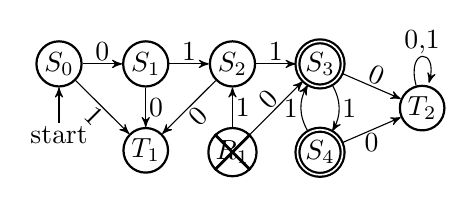
\begin{tikzpicture}[bezier bounding box,node distance=0.5cm]%reduce vertical space around graph
  \node[state, initial, initial where=below,minimum size=0.5cm] (s0) {$S_{0}$};
  \node[state, minimum size=0.5cm, right=of s0] (s1) {$S_{1}$};
  \node[state, minimum size=0.5cm, right=of s1] (s2) {$S_{2}$};
  \node[state, accepting, minimum size=0.5cm, right=of s2] (s3) {$S_{3}$};
  \node[state, accepting, minimum size=0.5cm, below=of s3] (s4) {$S_{4}$};
  \node[state, minimum size=0.5cm, below=of s1] (t2) {$T_{1}$};
  \node[state, minimum size=0.5cm, below=of s2] (r1) {$R_{1}$};

  % Calculate the midpoint between S3 and S4
  \coordinate (midpoint) at ($(s3)!0.5!(s4)$);

  \node[state, minimum size=0.5cm, right=1cm of midpoint] (t1) {$T_{2}$};
  \draw[black, line width=1pt] (r1.south west) -- (r1.north east);
  \draw[black, line width=1pt] (r1.north west) -- (r1.south east);

  \path[->]
  (s0) edge node[above]{0}(s1)
  (s0) edge node[below,sloped]{1}(t2)
  (s1) edge node[above]{1}(s2)
  (s1) edge node[right]{0}(t2)
  (s2) edge node[above]{1}(s3)
  (s2) edge node[below,sloped]{0}(t2)
  (s3) edge[bend left] node[right]{1}(s4)
  (s3) edge node[above,sloped]{0}(t1)
  (s4) edge node[below]{0}(t1)
  (s4) edge[bend left] node[left]{1}(s3)
  (r1) edge node[above,sloped]{0}(s3)
  (r1) edge node[right]{1}(s2)
  (t1) edge[loop above] node{0,1}(t1);
\end{tikzpicture}
\end{minipage}
}
\begin{enumerate}
\item \textbf{remove} any state unreachable from start state
\item \textbf{split} states into \textbf{final} group and \textbf{non-final} one
\item\label{dfa:mini} \textbf{find} where each state goes on some input
\item if 2 states with same input go to different groups, split out
\item repeat the step \ref{dfa:mini} until no splitting for any group
\end{enumerate}

Each of following has format: input [[states after input]]\\
\begin{minipage}{\linewidth}
  % Reduced vertical spacing
\setlength{\abovedisplayskip}{4pt}
\setlength{\belowdisplayskip}{4pt}
  \centering
\begin{align*}
& [[S_{0},S_{1},S_{2},T_{1},T_{2}],[S_{3},S_{4}]] && \leftarrow 0\quad \text{(init)}\\
& [[S_{0},S_{1},S_{2},T_{1},T_{2}],[S_{3},S_{4}]] && \leftarrow 1\\
& [[S_{0},S_{1},T_{1},T_{2}],[S_{2}],[S_{3},S_{4}]] && \leftarrow 0\\
& [[S_{0},T_{1},T_{2}],[S_{2}],[S_{3},S_{4}]] &&  \leftarrow 1\\
& [[S_{0},T_{1},T_{2}],[S_{1}],[S_{2}],[S_{3},S_{4}]] && \leftarrow 0\\
& [[T_{1},T_{2}],[S_{0}],[S_{1}],[S_{2}],[S_{3},S_{4}]] && \leftarrow 0\\
& [[T_{1},T_{2}],[S_{0}],[S_{1}],[S_{2}],[S_{3},S_{4}]] && \leftarrow 1
% & [[T_{1},T_{2}],[S_{0}],[S_{1}],[S_{2}],[S_{3},S_{4}]] && \leftarrow 1
\end{align*}
Thus, \(T_{1} \equiv T_{2}, S_{3} \equiv S_{4}\). New DFA diagram:
\end{minipage}

\begin{minipage}{0.9\linewidth}
  \centering
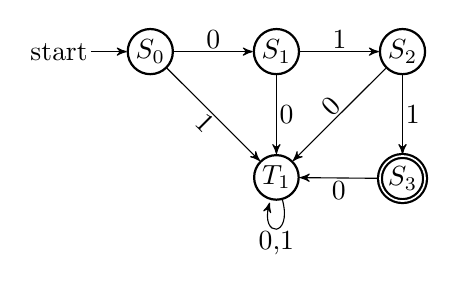
\begin{tikzpicture}[bezier bounding box,node distance=1cm]%reduce vertical space around graph
  \node[state, initial, minimum size=0.5cm] (s0) {$S_{0}$};
  \node[state, minimum size=0.5cm, right=of s0] (s1) {$S_{1}$};
  \node[state, minimum size=0.5cm, right=of s1] (s2) {$S_{2}$};
  \node[state, accepting, minimum size=0.5cm, below=of s2] (s3) {$S_{3}$};
  % \node[state, accepting, minimum size=0.5cm, below=of s3] (s4) {$S_{4}$};
  \node[state, minimum size=0.5cm, below=of s1] (t2) {$T_{1}$};
  % \node[state, minimum size=0.5cm, below=of s2] (r1) {$R_{1}$};

  \path[->]
  (s0) edge node[above]{0}(s1)
  (s0) edge node[below,sloped]{1}(t2)
  (s1) edge node[above]{1}(s2)
  (s1) edge node[right]{0}(t2)
  (s2) edge node[right]{1}(s3)
  (s2) edge node[above,sloped]{0}(t2)
  (s3) edge node[below]{0}(t2)
  (t2) edge[loop below] node{0,1}(t2);
\end{tikzpicture}
\end{minipage}


\section*{Grammar Tuple}
\begin{minipage}{0.45\linewidth}
\begin{enumerate}
\item \(terminals\): finite set of symbols forming strings of defined language
\item \(S(G) \overset{*}{\Rightarrow} w\): \emph{start symbole} derives \emph{w} by \(G\) in 0/more steps
\item a \emph{w}ord contains ONLY \emph{terminals}
\item a \emph{sentential form} MUST contain 1 or more \emph{vars} (e.g. \(aSb\))
\item \emph{leftmost derivation}: always replace leftmost var by 1 of \(P\)s
\end{enumerate}
\end{minipage}
{\footnotesize
\begin{minipage}{0.5\linewidth}
  \centering
  \begin{tabular}{r|l}
    & $G = (V,T,P,S)$  \\
    \hline
    $V$ & $V_{t} \cup V_{n}$ \\
    $T$ & $\mathsf{terminals} \; (V_{t})$\\
    $P$ & $\mathsf{productions}$ \\
    $S$ & $\mathsf{start \; symbol}$\\
    \hline
\end{tabular}\\
Design/find a grammar is to give the above tuple.\\
Example: equal number of \(a, b\):
\[
  G = (\{a,T,b\},\{T\},\{T \rightarrow aTb \gor \epsilon\},T)
\]

\end{minipage}
}


\section*{Parse Trees and (un)ambiguity}
\begin{minipage}{0.45\linewidth}
  % Reduced vertical spacing
\setlength{\abovedisplayskip}{0pt}
\setlength{\belowdisplayskip}{0pt}
\begin{enumerate}
\item left/right associativity:
  \[
    S \rightarrow S - S \Rightarrow\left\{
      \begin{array}{l}
        S \rightarrow S - \mathsf{int} \\
        S \rightarrow \mathsf{int} - S
      \end{array}
       \right.
  \]
\item higher precedence: the \(V_{n}\) \textbf{closer} to \(V_{t}\) or use \verb|()|
  \begin{itemize}[leftmargin=1.5em]
    \item[$P_{1}$] \(S \rightarrow S + T \gor T\)
    \item[] ``+'' can't break \(T\)
    \item[$P_{2}$] \(T \rightarrow T * \mathsf{int} \gor \mathsf{int}\)
    \item[] positioned lower than \(P_{1}\)
    \item \(P_{2}\) has \textbf{higher} priority: always expand \(T\) first
    \end{itemize}
\item Controlling \(\epsilon\) (only derived from \(S\)):
  \[
    S \rightarrow \epsilon \gor (S) \gor SS \Rightarrow\left\{
        \begin{array}{l}
          S \rightarrow \epsilon \gor T\\
          T \rightarrow TU \gor U\\
          U \rightarrow () \gor U \rightarrow (T)
        \end{array}
      \right.
  \]
\end{enumerate}
\end{minipage}
\begin{minipage}[t]{0.45\linewidth}
  \centering
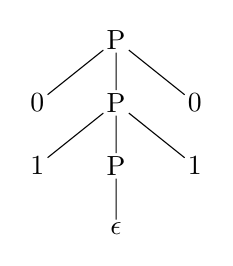
\begin{tikzpicture}[level distance=8mm,level/.style={sibling distance=10mm}]
  \node {P}
  child {node {0}}
  child {
    node {P}
    child {node {1}}
    child {
      node {P}
      child {node {\(\epsilon\)}}
    }
    child {node {1}}
  }
  child {node {0}};
\end{tikzpicture}\\
\emph{un}ambiguous grammar: \textbf{unique} parse tree of given string.  Concatenate leaves (\(V_{t}/\epsilon\)) of a parse tree \textbf{anti-clockwise} and get the \textbf{yield} of the parse tree: \textbf{0110}
\end{minipage}


\section*{Regular (Type-3) \& Context-free (Type 3)}
\begin{minipage}[t]{0.5\linewidth}
  \textbf{Context-free grammar}\\
\(\forall p \in P: A \rightarrow w\) where
\begin{itemize}
\item \(A \in V_{n}\) and \(w \in V^{*}\) is an arbitrary string
\item \(A\) (\textbf{left} of each \(p \in P\)) must be a \textbf{single non-terminal}
\item right-side can be anything
\item free of content, LHS can replace RHS
\end{itemize}
\end{minipage}
\begin{minipage}[t]{0.5\linewidth}
  \textbf{Context-free grammar}
\begin{itemize}
\item \emph{regular} means any \(p \in P\) is \emph{right}-linear or \emph{left}-linear
  \begin{itemize}[leftmargin=3em]
  \item[right] \(A \rightarrow aB \gor a \gor \epsilon\) \textbf{(focus)}
  \item[left] \(A \rightarrow Ba\ \gor a \gor \epsilon\)
  \end{itemize}
\item right-linear == left-linear
\item If \(A \derive{*}{lm} w\) AND \(A \derive{*}{rm} w\), THEN \(A \overset{*}{\Rightarrow} w\)
\item terminate with terminals or \(\epsilon\)
\end{itemize}
\end{minipage}


\section*{Pushdown Automata (PDA)}
{\footnotesize
\begin{minipage}[]{0.5\linewidth}
  \[\delta\overbracket[1pt]{(q,a,X)}^\text{3 args} \overset{*}{\mapsto} \overbracket{(p,\gamma)}^\text{2 outputs} \]
  $\delta$ is partial: undefined for some input \(\notin \Sigma\)
\begin{enumerate}
 \item $q$ a state \(\in Q\)
 \item $a$ an input string of symbol(s) \(\in \Sigma\) or \(a = \epsilon\)
 \item $X$ a stack symbol \(\in \Gamma \)
 \item $p$ new state \(p \in Q\)
 \item $\gamma$ string of stack symbols replacing $X$
   \begin{enumerate}
     \item $\gamma = \epsilon$, stack popped
     \item $\gamma = X$, stack unchanged
     \item $\gamma = YZ$, $X$ replaced by $Z$ and $Y$ is pushed
  \end{enumerate}
\end{enumerate}
\end{minipage}
\begin{minipage}{0.45\linewidth}
  \centering
  \begin{tabular}{r|p{3.8cm}}
    & $P = (Q,\Sigma,\Gamma,\delta,q_{0},Z_{0},F)$  \\
    \hline
    $Q$ & set of \emph{states}\\
    $\Sigma$ & set of \emph{input symbols}\\
    $\Gamma$ & set of allowed \emph{stack alphabet}\\
    $\delta$ & \emph{transition function}\\
    $q_{0}$  &  set of \emph{states}\\
    $Z_{0}$  & set of \emph{states}\\
    $F$      & set of \(accepting/final\; states\)\\
    \hline
    \multicolumn{2}{l}{all above sets are \textbf{finite}: \(F \subseteq Q\) }\\
    \multicolumn{2}{l}{define/recog. all and only CFG}\\
    \hline
  \end{tabular}
\vskip 1em
PDA is essentially an \(\epsilon\)-NFA with an additional stack
\end{minipage}
}


\section*{Derive NPDA for CFG and Trace}
% Steps 1-2
{\footnotesize
\begin{minipage}{\linewidth}
\begin{enumerate}
\item \textbf{initialize} See empty stack \(Z\) and push \(S\)
\item[] \(\delta(q_{0},\epsilon,Z) \mapsto q_{1}/\mathbf{S}Z\)
\item \textbf{expand non-terminals}: input = \(\epsilon\)
\end{enumerate}
\end{minipage}
\begin{minipage}[t]{0.45\linewidth}
  \setlength{\abovedisplayskip}{1pt}
  \setlength{\belowdisplayskip}{1pt}
  \begin{align*}
   \delta(q_{1},\epsilon,\mathbf{S})& \mapsto q_{1}/S+T\\
   \delta(q_{1},\epsilon,\mathbf{S})& \mapsto q_{1}/T\\
   \delta(q_{1},\epsilon,\mathbf{T})& \mapsto q_{1}/T * U\\
   \delta(q_{1},\epsilon,\mathbf{T})& \mapsto q_{1}/U\\
   \delta(q_{1},\epsilon,\mathbf{U})& \mapsto q_{1}/(S)\\
   \delta(q_{1},\epsilon,\mathbf{U})& \mapsto q_{1}/\mathsf{int}
  \end{align*}
\end{minipage}
% Given CFG
\begin{minipage}[t]{0.45\linewidth}
\begin{align*}
  S &\rightarrow S + T \gor T\\
  T &\rightarrow T * U \gor U\\
  U &\rightarrow (S) \gor \mathsf{int}
\end{align*}
Given (if \(L(P)\), convert it to) CFG, derive its PDA
\end{minipage}
% Steps 3-4
\begin{minipage}[t]{0.4\linewidth}
\begin{enumerate}[resume,start=3]
\item \textbf{match \& pop \(V_{t}\)}
\item[] input \(\in V_{t}\)
  \begin{align*}
  \delta&(q_{1},\mathbf{+},\mathbf{+})& \mapsto &\quad q_{1}/\epsilon\\
  \delta&(q_{1},\mathbf{*},\mathbf{*})& \mapsto &\quad q_{1}/\epsilon\\
  \delta&(q_{1},\mathsf{int},\mathsf{int})& \mapsto &\quad q_{1}/\epsilon\\
  \delta&(q_{1},\mathbf{(},\mathbf{(})& \mapsto &\quad q_{1}/\epsilon\\
  \delta&(q_{1},\mathbf{)},\mathbf{)})& \mapsto &\quad q_{1}/\epsilon
  \end{align*}
\item \textbf{terminate} $\delta(q_{1},\epsilon,Z) \mapsto q_{2}/\epsilon$
\end{enumerate}
\end{minipage}
% Exampel trace
\begin{minipage}[t]{0.55\linewidth}
\setlength{\abovedisplayskip}{-1em}
\setlength{\belowdisplayskip}{0pt}
  \begin{align*}
    & (q_{1},\mathsf{int * int}, \mathbf{Z}) \Rightarrow (q_{1}, \mathsf{int * int}, SZ)\\
    &\Rightarrow (q_{1}, \mathsf{int * int}, TZ)\\
    &\Rightarrow (q_{1}, \mathsf{int * int}, T*UZ)\\
    &\Rightarrow (q_{1}, \mathsf{int * int}, U*UZ)\\
    &\Rightarrow (q_{1}, \mathsf{int * int}, \mathsf{int}*UZ)\\
    &\Rightarrow (q_{1}, \mathsf{ * int}, *UZ)\\
    &\Rightarrow (q_{1}, \mathsf{int}, UZ)\\
    &\Rightarrow (q_{1}, \mathsf{int}, \mathsf{int}Z)\\
    &\Rightarrow (q_{1}, \epsilon, Z) \Rightarrow (q_{1}, \epsilon, \epsilon) accpet\\
  \end{align*}
\end{minipage}
}


\section*{Turing Machine (TM)}
{\footnotesize
\begin{minipage}[]{0.45\linewidth}
  \[\delta\overbracket[1pt]{(q,a,X)}^\text{3 args} \overset{*}{\mapsto} \overbracket{(p,\gamma)}^\text{2 outputs} \]
  $\delta$ is partial: undefined for some input \(\notin \Sigma\)
\begin{enumerate}
    \item \(q\) current state, \(q \in Q\)
    \item \(X\) current tape symbol, \(X \in \Gamma\)
    \item \(p\) next state, \(p \in Q\), from \(q\), through 0/more moves, to \(q\)
    \item \(Y \in \Gamma\), symb in tape cell, replacing whatever was there
    \item \(D\) \emph{direction}, \(L \leftarrow\), \(R \rightarrow\) or \(S\) (stay/halt)
    \item if \(L = L(M)\) accpt. by some TM \(M\), \(L\) is \emph{recursively enumerable}
\end{enumerate}
\end{minipage}
\begin{minipage}{0.5\linewidth}
  \centering
  \begin{tabular}{r|p{3.8cm}}
    & $ M = (Q,\Sigma,\Gamma,\delta,q_{0},B,F)$  \\
    \hline
    $Q$ & set of \emph{states} of finite ctrl\\
    $\Sigma$ & finite set of \emph{input symbols}: \(\Sigma \subset \Gamma\)\\
    $\Gamma$ & complete set of \emph{tape symbols}\\
    $\delta$ & \emph{transition function}\\
    $q_{0}$  &  \emph{start state} \(\in Q\)\\
    $B$     & \emph{blank} symbol$^{2}$, also \(\Lambda\)\\
    $F$      & set of \emph{final} or \emph{accepting} states: \(F \subset Q\)\\
    \hline
    \multicolumn{2}{l}{all above sets are \textbf{finite}: \(F \subseteq Q\) }\\
    \hline
\end{tabular}\\
\end{minipage}
}

{\footnotesize
% Increment
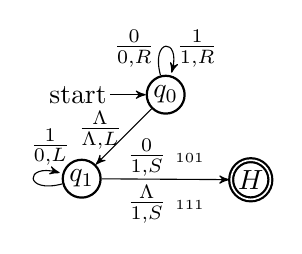
\begin{tikzpicture}[bezier bounding box]%reduce vertical space around graph
  \node[state, initial, minimum size=1em] (q0) {$q_0$};
  \node[state, minimum size=1em, below left=of q0] (q1) {$q_1$};
  \node[state, accepting, minimum size=1em, below right=of q0] (h) {$H$};

  \path[->] (q0)
  edge[loop above]
  node[yshift=-0.3cm,xshift=-0.4cm]{$\frac{0}{0,R}$}
  node[yshift=-0.3cm,xshift=0.4cm]{$\frac{1}{1,R}$} (q0)

  edge[above] node[yshift=-0.2cm,xshift=-0.3cm]{$\frac{\Lambda}{\Lambda,L}$} (q1)

  (q1) edge[loop left] node[yshift=0.4cm,xshift=0.5cm]{$\frac{1}{0,L}$}
  (q1) edge[above]
  node[yshift=-0.6cm]{$\frac{\Lambda}{1,S}$ \tiny111}
  node{$\frac{0}{1,S}$ \tiny101}(h);
\end{tikzpicture}
% Decrement
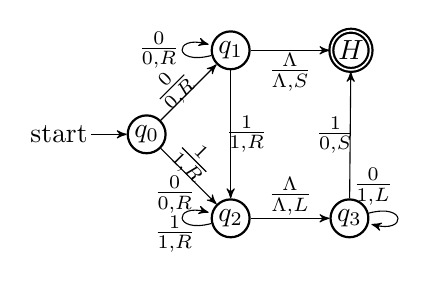
\begin{tikzpicture}[bezier bounding box]%reduce vertical space around graph
  \node[state, initial, minimum size=1em] (q0) {$q_0$};
  \node[state, minimum size=1em, above right=of q0] (q1) {$q_1$};
  \node[state, minimum size=1em, below right=of q0] (q2) {$q_2$};
  \node[state, minimum size=1em, right=of q2] (q3) {$q_3$};
  \node[state, accepting, minimum size=1em, right=of q1] (h) {$H$};

  \path[->]
  (q0)
  edge node[above,sloped,yshift=-0.1cm,xshift=-0.1cm]{$\frac{0}{0,R}$}(q1)
  edge node[above,sloped,yshift=-0.1cm,xshift=-0.1cm,]{$\frac{1}{1,R}$}(q2)

  (q1)
  edge[loop left] node{$\frac{0}{0,R}$}(q1)
  edge[below] node{$\frac{\Lambda}{\Lambda,S}$}(h)
  edge node[right,xshift=-0.1cm]{$\frac{1}{1,R}$}(q2)

  (q2)
  edge[loop left]
  node[yshift=0.3cm,xshift=0.2cm]{$\frac{0}{0,R}$}
  node[yshift=-0.2cm,xshift=0.2cm]{$\frac{1}{1,R}$}(q2)
  edge[above] node{$\frac{\Lambda}{\Lambda,L}$}(q3)

  (q3)
  edge[loop right] node[yshift=0.4cm,xshift=-0.6cm]{$\frac{0}{1,L}$}(q3)
  edge node[left,xshift=0.1cm]{$\frac{1}{0,S}$}(h);
\end{tikzpicture}\\
\(TM\) for inc bin num by 1 \hfill \(TM\) for dec bin num by 1\\
}


\section*{Hoare logic}
\begin{enumerate}
\item \textbf{Weak} pre/post-conditions: more \textbf{general} (say \emph{less})
\item \textbf{Weakest} possible: \textbf{\texttt{True}}
\item \textbf{Strongest} possible: \textbf{\texttt{False}}
\item \textbf{Strong} pre/post-conditions: more \textbf{specific} (say \emph{more})
\item Usually want to find \textbf{weakest precondition} $Q_{wp}$ (more general and allow more input).
\end{enumerate}

\subsection*{1/6 Assignment Rule}
\(\qquad\{?\}\ i := 2 * i \{i < 6\}\)\hfill\(\{x > 3\}\;x:=x+2\;\{x>5\}\)\\
\begin{minipage}{0.5\linewidth}
\begin{enumerate}
\item \textbf{copy} Q over to P: \(\{i_{post} < 6\}\)
\item \textbf{replace} all LHS vars with RHS in assignment(s): \(\{2 * i < 6\}\)
\item See if any math/logic equivalence: \(\{i_{orig} < 3\}\)
\end{enumerate}
\end{minipage}
\begin{minipage}{0.5\linewidth}
\begin{enumerate}
\item \textbf{copy} Q over to P: \(\{x_{post} > 5\}\)
\item \textbf{replace} all LHS vars with RHS vars: \(\{x_{assign}+2 > 5\}\)
\item \textbf{find} if any math/logic equivalence: \(\{x_{orig} > 3\}\)
\end{enumerate}
\end{minipage}

\subsection*{2/6 Pre-condition Strengthening}
\begin{displaymath}
  \frac{P_{strong} \rightarrow P_{weak} \quad \{P_{weak}\}\,S\,\{Q\} } {\{P_{strong}\}\,S\,\{Q\}}
\end{displaymath}

\subsection*{3/6 Post-condition Weakening}
\begin{displaymath}
  \frac{Q_{strong}\rightarrow Q_{weak} \quad \{P\}\,S\,\{Q_{strong}\} } {\{P\}\,S\,\{Q_{weak}\}}
\end{displaymath}

\subsection*{4/6 Sequencing}
\begin{displaymath}
  \frac{\{P\}\,S_{1}\,\{ Q_{mid}\}\ \quad \{Q_{mid}\}\,S_{2}\,\{R\}}{\{P\}\,S\,\{R\}}
\end{displaymath}
\begin{enumerate}
\item $Q_{mid}$ \textbf{weak} enough such that $P$ to $Q_{mid}$ holds
\item[] strengthen precond. $W_{sp} \rightarrow Q_{mid}$, if $W_{sp}$ then $Q_{mid}$
\item $Q_{mid}$ \textbf{strong} enough such that $P$ to $Q$ holds
\item[] weaken post $Q_{mid} \rightarrow W_{wp}$, if $W$, then $Q_{mid}$
\item Assignment rule backwards to find proper $Q_{mid}$
\end{enumerate}
% \subsection*{Question Type}
% {
%   % Reducing vertical spacing
%   \setlength{\abovedisplayskip}{0pt}
%   \setlength{\belowdisplayskip}{3pt}
%   \setlength{\abovedisplayshortskip}{0pt}
%   \setlength{\belowdisplayshortskip}{3pt}
%
%   \[\textbf{Prove:}\quad \{P\}\,S_{1};\,S_{2};\,\ldots ;\,S_{n}\,\{Q\}\]
% }
% \textbf{Solution} Start backwards and use Assignment Rule:
% \begin{enumerate}
% \item\label{step1} \textbf{Copy} \(Q_{n}\) as \(P_{n}\) for \(S_{n}\)
% \item\label{step2} \textbf{Use} assignment rule and math equivalence to simplify \(P_{n}\) if possible
% \item \textbf{Use} \(P_{n}\) as \(P_{n-1}\) for \(S_{n-1}\)
% \item \textbf{Repeat} \ref{step1} and \ref{step2} until getting \(P_{1}\)
% \item \textbf{Strengthen} precondition \(\{P\}\rightarrow \{P_{1}\}\)
% \item (Optional) Sometimes need (0th/boolean) logic to simplify compound propositions.
%
% \end{enumerate}

\subsection*{5/6 Conditionals}
\begin{displaymath}
  \frac{\{P \land\; b\}\;S_{1}\{Q\} \quad \{P \land \;\neg b\}\;S_{2}\;\{Q\}}{\{P\}\;\texttt{if}\;b\;S_{1}\;\texttt{then}\;S_{2}\;\{Q\}}
\end{displaymath}
% {
%   % Reducing vertical spacing
%   \setlength{\abovedisplayskip}{0pt}
%   \setlength{\belowdisplayskip}{3pt}
%   \setlength{\abovedisplayshortskip}{0pt}
%   \setlength{\belowdisplayshortskip}{3pt}
%
% \[\textbf{Prove:}\quad \{P\}\;if\:b\:then\:S_{1}\:else\:S_{2}\;\{Q\}\]
% }

\subsection*{Complete conditionals}
Conditionals with \texttt{else} branch are \emph{complete}.

\texttt{if b then S} $\Longleftrightarrow$ \texttt{if b then S else (do nothing)}
\begin{displaymath}
  \frac{\{P \land\; b\}\;S\{Q\} \quad \{P \land \;\neg b\}\;\texttt{(do nothing)}\;\{Q\}}{\{P\}\;\texttt{if}\;b\;\texttt{then}\;S\;\{Q\}}
\end{displaymath}
\texttt{do nothing} can be \textbf{strengthened} to sth like \verb|x := x|

\subsection*{6/6 While Loop}
\begin{displaymath}
  \frac{\{I \land\; b\}\;S\;\{I\}}{\{I\}\;\texttt{while}\;b\;\texttt{do}\;S\;\{I \land\l \neg b\}}
\end{displaymath}
\begin{enumerate}
\item \textbf{invariant} often looks similar to final $S$
\item \textbf{invariant} may be an equation plus restraints
\item \textbf{variant} often looks simiar to loop condition $b$
\end{enumerate}


\end{multicols*}
\end{document}
